%%%%%%%%%%%%%%%%%%%%%%%%%%%%%%%%%%%%%%%%%
% Short Sectioned Assignment
% LaTeX Template
% Version 1.0 (5/5/12)
%
% This template has been downloaded from:
% http://www.LaTeXTemplates.com
%
% Original author:
% Frits Wenneker (http://www.howtotex.com)
%
% License:
% CC BY-NC-SA 3.0 (http://creativecommons.org/licenses/by-nc-sa/3.0/)
%
%%%%%%%%%%%%%%%%%%%%%%%%%%%%%%%%%%%%%%%%%

%----------------------------------------------------------------------------------------
%	PACKAGES AND OTHER DOCUMENT CONFIGURATIONS
%----------------------------------------------------------------------------------------

\documentclass[norsk]{article} % A4 paper and 11pt font size

\usepackage[T1]{fontenc} % Use 8-bit encoding that has 256 glyphs
\usepackage{fourier} % Use the Adobe Utopia font for the document - comment this line to return to the LaTeX default
\usepackage[english]{babel} % English language/hyphenation
\usepackage{amsmath,amsfonts,amsthm} % Math packages

% Added by Haavard %---------------------------------------------------------------------
\usepackage[utf8]{inputenc} % Norwegian letters
\usepackage{fullpage}
\usepackage{subcaption}
\usepackage[font={small, it}]{caption} % captions on figures and tables
\usepackage{graphicx}
% --------------------------------------------------------------------------------------

\usepackage{lipsum} % Used for inserting dummy 'Lorem ipsum' text into the template

\usepackage{sectsty} % Allows customizing section commands
\allsectionsfont{\centering \normalfont\scshape} % Make all sections centered, the default font and small caps

\usepackage{fancyhdr} % Custom headers and footers
\pagestyle{fancyplain} % Makes all pages in the document conform to the custom headers and footers
\fancyhead{} % No page header - if you want one, create it in the same way as the footers below
\fancyfoot[L]{} % Empty left footer
\fancyfoot[C]{} % Empty center footer
\fancyfoot[R]{\thepage} % Page numbering for right footer
\renewcommand{\headrulewidth}{0pt} % Remove header underlines
\renewcommand{\footrulewidth}{0pt} % Remove footer underlines
\setlength{\headheight}{13.6pt} % Customize the height of the header

\numberwithin{equation}{section} % Number equations within sections (i.e. 1.1, 1.2, 2.1, 2.2 instead of 1, 2, 3, 4)
\numberwithin{figure}{section} % Number figures within sections (i.e. 1.1, 1.2, 2.1, 2.2 instead of 1, 2, 3, 4)
\numberwithin{table}{section} % Number tables within sections (i.e. 1.1, 1.2, 2.1, 2.2 instead of 1, 2, 3, 4)

\setlength\parindent{0pt} % Removes all indentation from paragraphs - comment this line for an assignment with lots of text

%----------------------------------------------------------------------------------------
%	TITLE SECTION
%----------------------------------------------------------------------------------------

\newcommand{\horrule}[1]{\rule{\linewidth}{#1}} % Create horizontal rule command with 1 argument of height

\title{	
\normalfont \normalsize 
\textsc{NTNU} \\ [25pt] % Your university, school and/or department name(s)
\horrule{0.5pt} \\[0.4cm] % Thin top horizontal rule
\huge TMA4280 - project part 2\\ % The assignment title
\horrule{2pt} \\[0.5cm] % Thick bottom horizontal rule
}

\author{Håvard Kvamme, Jørgen Vågan, Magnus Aarskaug Rud} % Your name

\date{\normalsize\today} % Today's date or a custom date

\begin{document}

\maketitle % Print the title

%----------------------------------------------------------------------------------------
%	PROBLEM 1
%----------------------------------------------------------------------------------------
\abstract{In this project the Kongull cluster have been used to solve the homogenous 
					2D Poisson problem on the unit square, both Message sending and shared memory 
				  solution models have been implemented and compared}

\section{Problem Description}
Poisson blabla 

\subsection{Kongull cluster}
Data specifications

\section{Solution}
General approach to the solution, FST 

\subsection{Implementation strategy}
More detailled: Transposing - MPI - OpenMP

\section{Results}
Presentation of graphs, vary p from 1 to 36
and $n= 2^{14}$

\begin{figure}[h!]
  \centering
  \begin{subfigure}[b]{0.48\textwidth}
    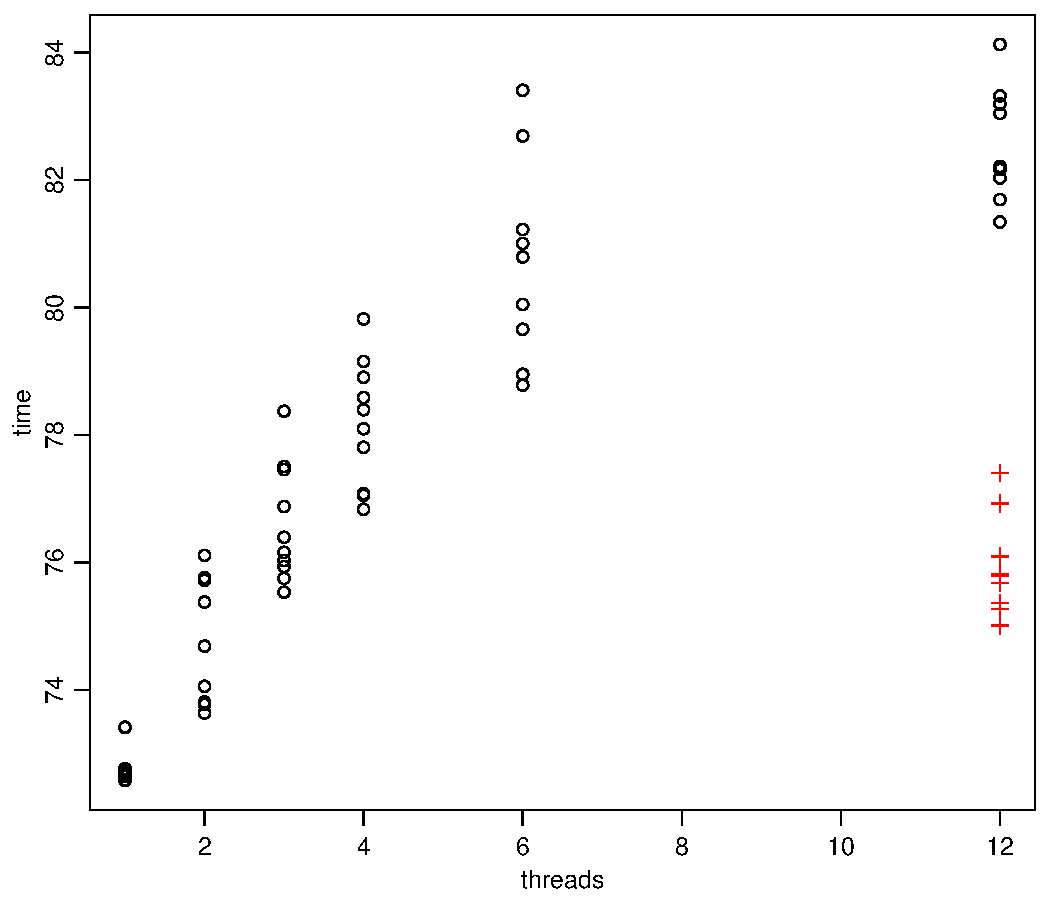
\includegraphics[width=\textwidth]{./Figures/taskc1.pdf}
  \end{subfigure}%
  \quad
  \begin{subfigure}[b]{0.48\textwidth}
    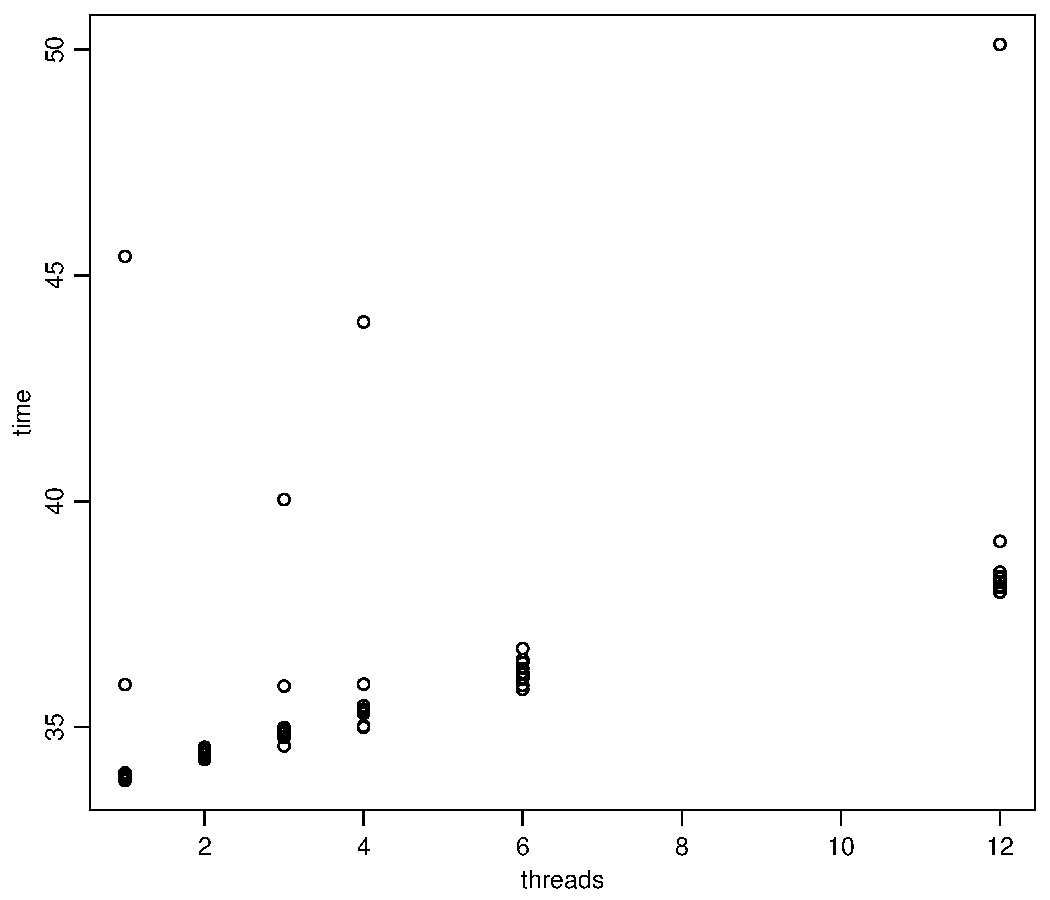
\includegraphics[width=\textwidth]{./Figures/taskc2.pdf}
  \end{subfigure}
          %(or a blank line to force the subfigure onto a new line)
  \vspace{1\baselineskip}
  \caption{Times (in seconds) for running MPI processes vs threads with $n = 2^{14}$. The total number of processors used are 12 per node, so the number of processes per node is 12 - threads. The left figure is run on one node, while the right is run on three nodes. The red crosses are run without any MPI sending at all.}
  \label{fig:taskc}
\end{figure}
%
\begin{figure}[h!]
  \centering
  \begin{subfigure}[b]{0.48\textwidth}
    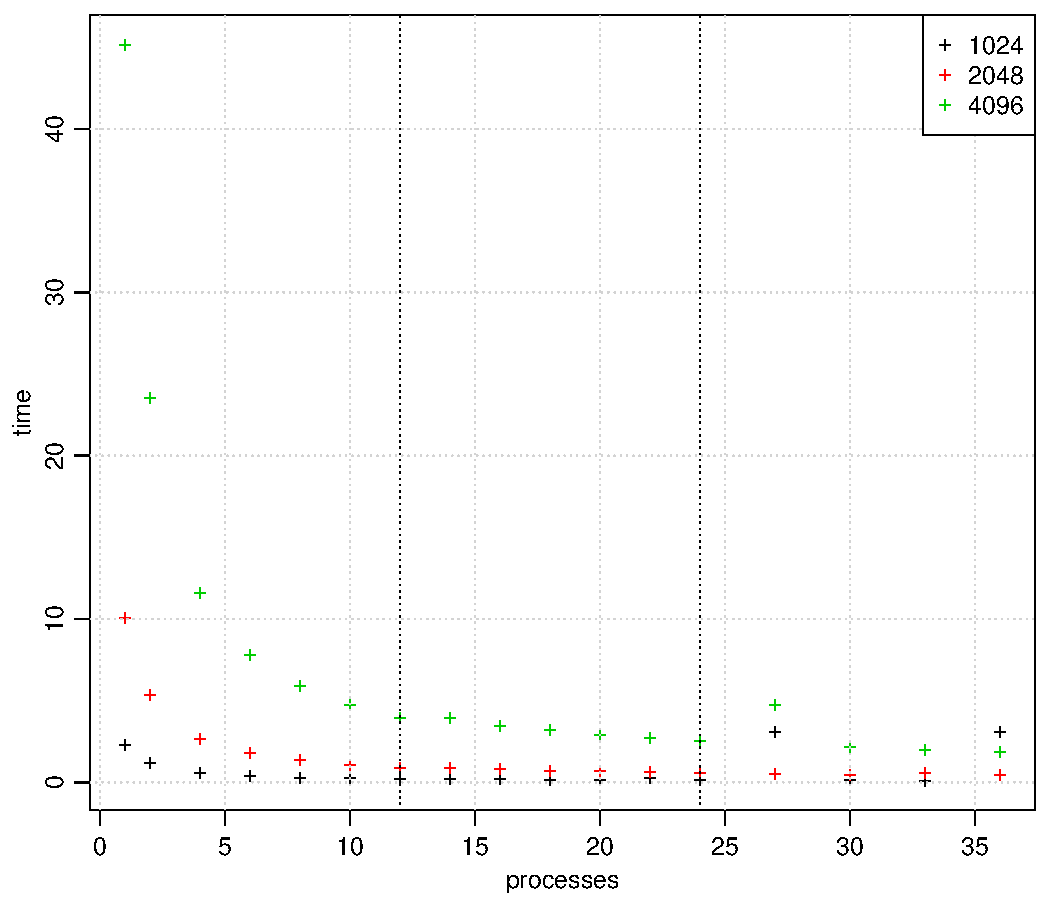
\includegraphics[width=\textwidth]{./Figures/taskbTimeProc1.pdf}
  \end{subfigure}%
  \quad
  \begin{subfigure}[b]{0.48\textwidth}
    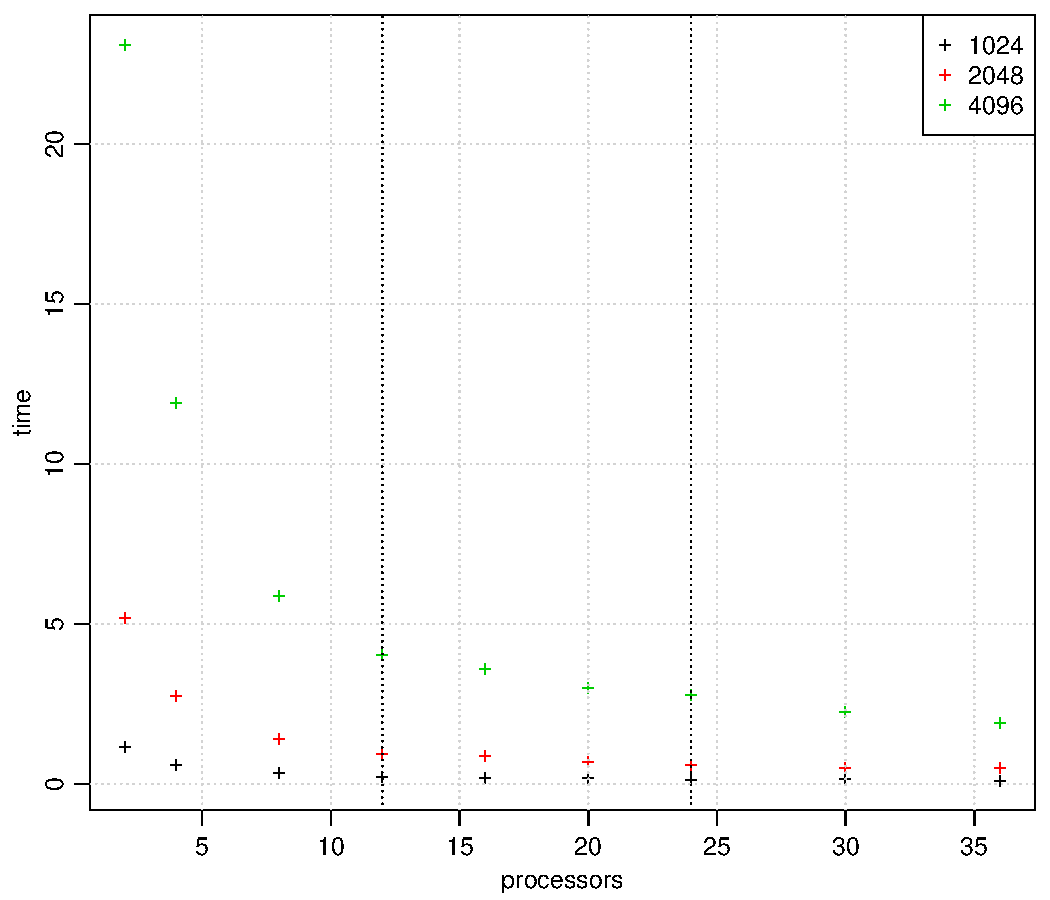
\includegraphics[width=\textwidth]{./Figures/taskbTimeProc2.pdf}
  \end{subfigure}
  \quad
  \begin{subfigure}[b]{0.48\textwidth}
    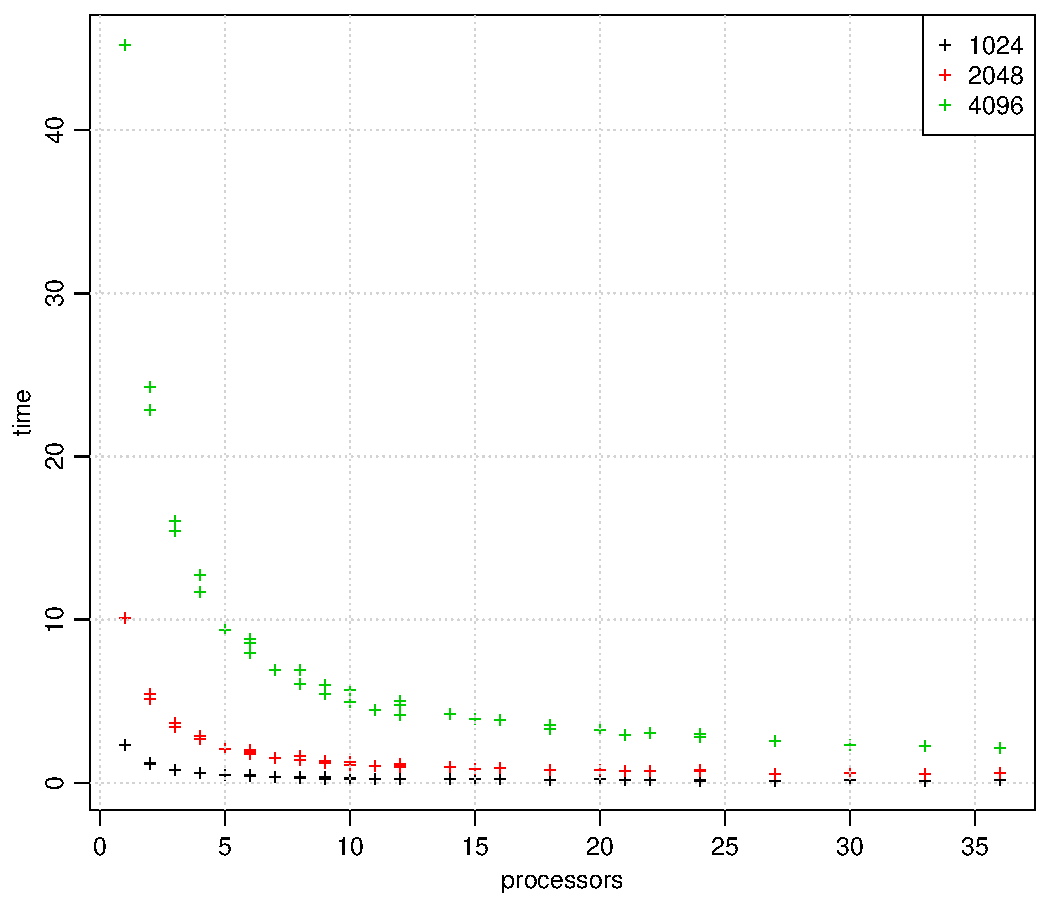
\includegraphics[width=\textwidth]{./Figures/taskbTimeNodesTimesThreads.pdf}
  \end{subfigure}
          %(or a blank line to force the subfigure onto a new line)
  \vspace{1\baselineskip}
  \caption{Times for running problem with different amount of processes. In the upper left figure each process has one thread, while in the upper right, each process has two treads. The problem is run on as few nodes as possible, and the processes are identically distributed among the nodes. The problem size $n$ is specified in the plots. In the bottom figure only one MPI process is run per node. Between 1 and 12 threads are run on each node.}
  \label{fig:time}
\end{figure}
%
\begin{figure}[h!]
  \centering
  \begin{subfigure}[b]{0.48\textwidth}
    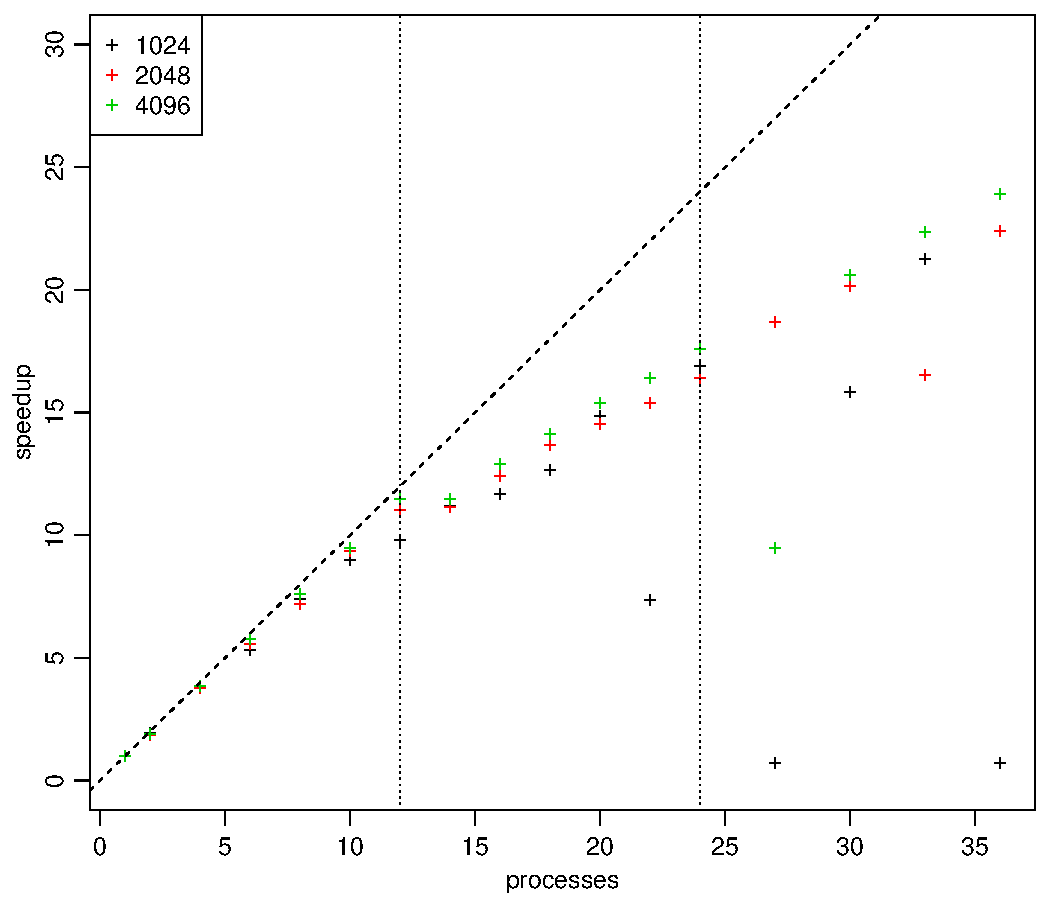
\includegraphics[width=\textwidth]{./Figures/taskbSpeedupProc1.pdf}
  \end{subfigure}%
  \quad
  \begin{subfigure}[b]{0.48\textwidth}
    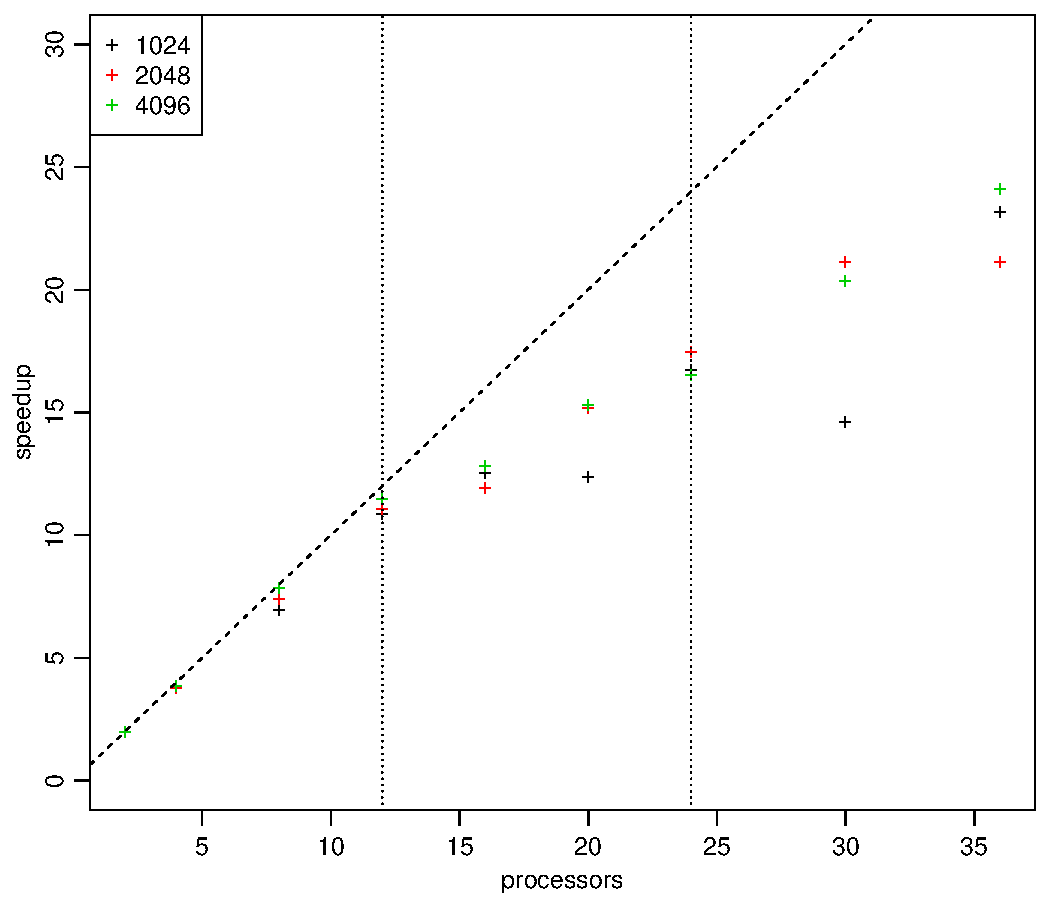
\includegraphics[width=\textwidth]{./Figures/taskbSpeedupProc2.pdf}
  \end{subfigure}
  \quad
  \begin{subfigure}[b]{0.48\textwidth}
    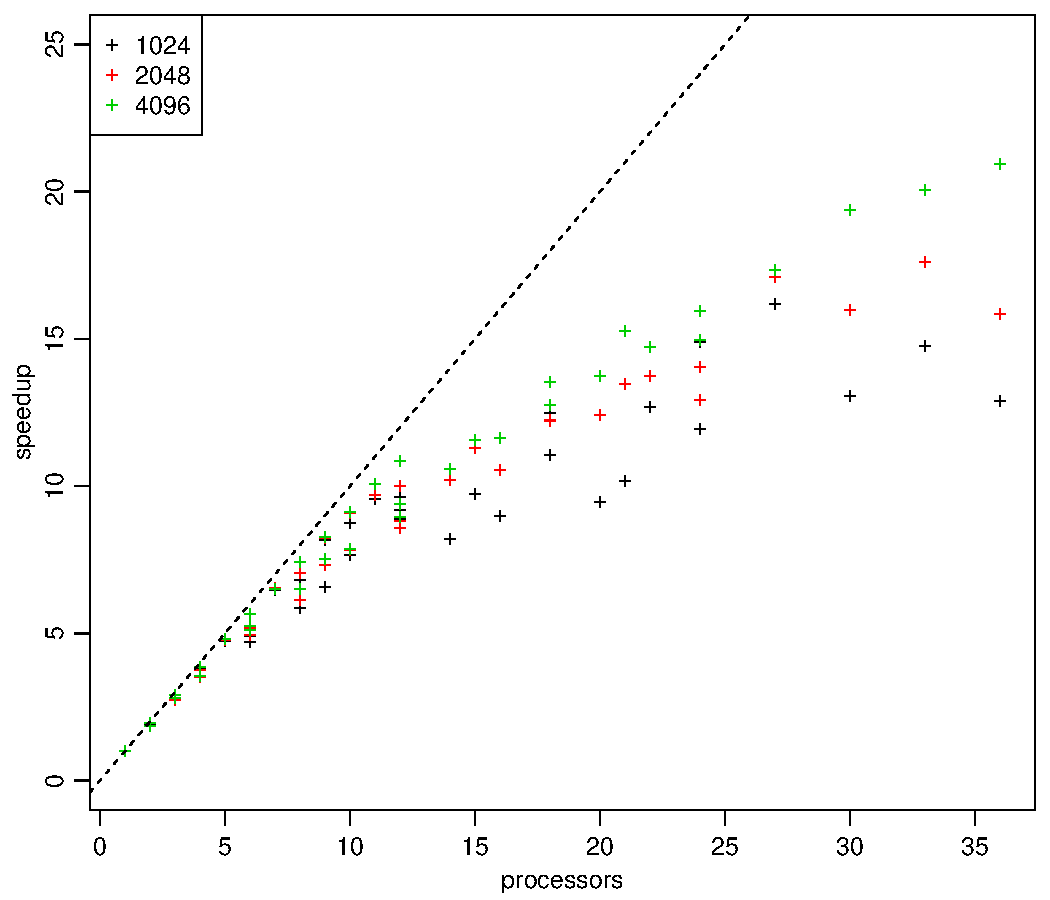
\includegraphics[width=\textwidth]{./Figures/taskbSpeedupNodesTimesThreads.pdf}
  \end{subfigure}
          %(or a blank line to force the subfigure onto a new line)
  \vspace{1\baselineskip}
  \caption{Speedup for running problem with different amount of processes. In the upper left figure each process has one thread, while in the upper right, each process has two treads. The problem is run on as few nodes as possible, and the processes are identically distributed among the nodes. There are drawn vertical lines to show when a new node is utilized, and a line with slope 1. The problem size $n$ is specified in the plots. In the bottom figure only one MPI process is run per node. Between 1 and 12 threads are run on each node.}
  \label{fig:Speedup}
\end{figure}
%
\begin{figure}[h!]
  \centering
  \begin{subfigure}[b]{0.48\textwidth}
    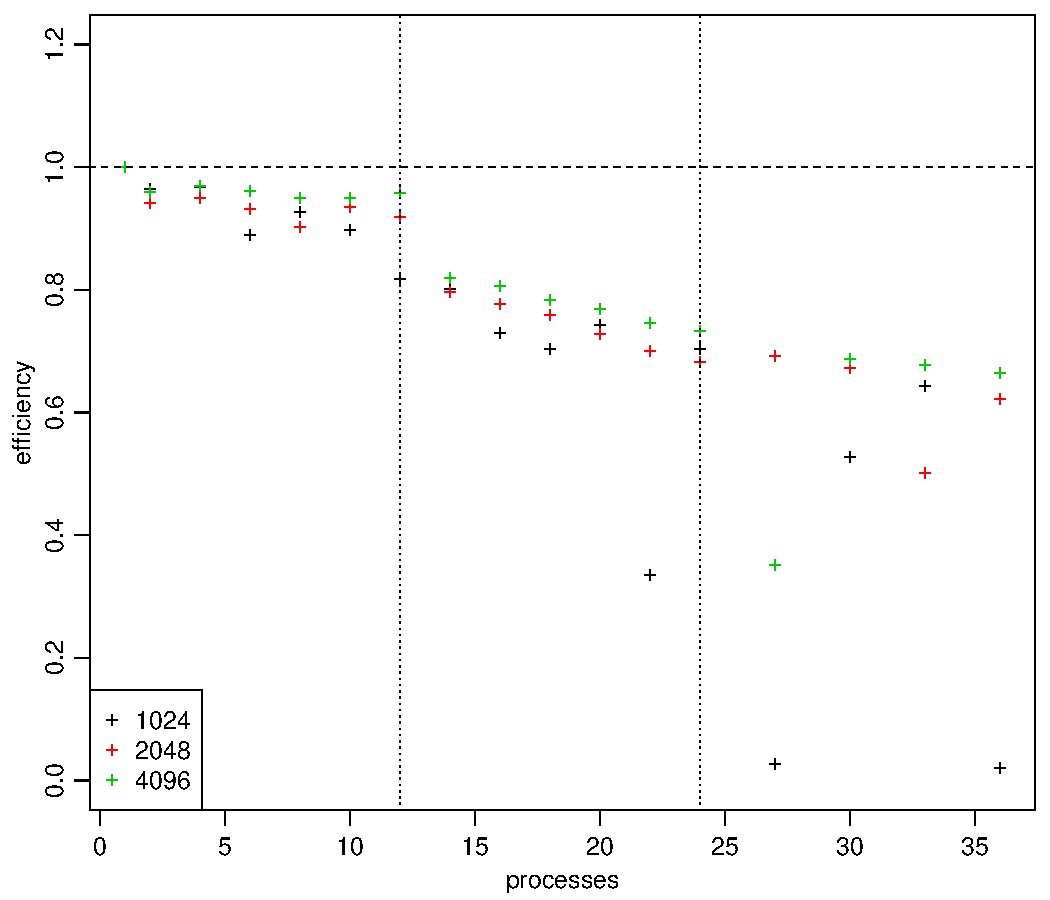
\includegraphics[width=\textwidth]{./Figures/taskbEfficiencyProc1.pdf}
  \end{subfigure}%
  \quad
  \begin{subfigure}[b]{0.48\textwidth}
    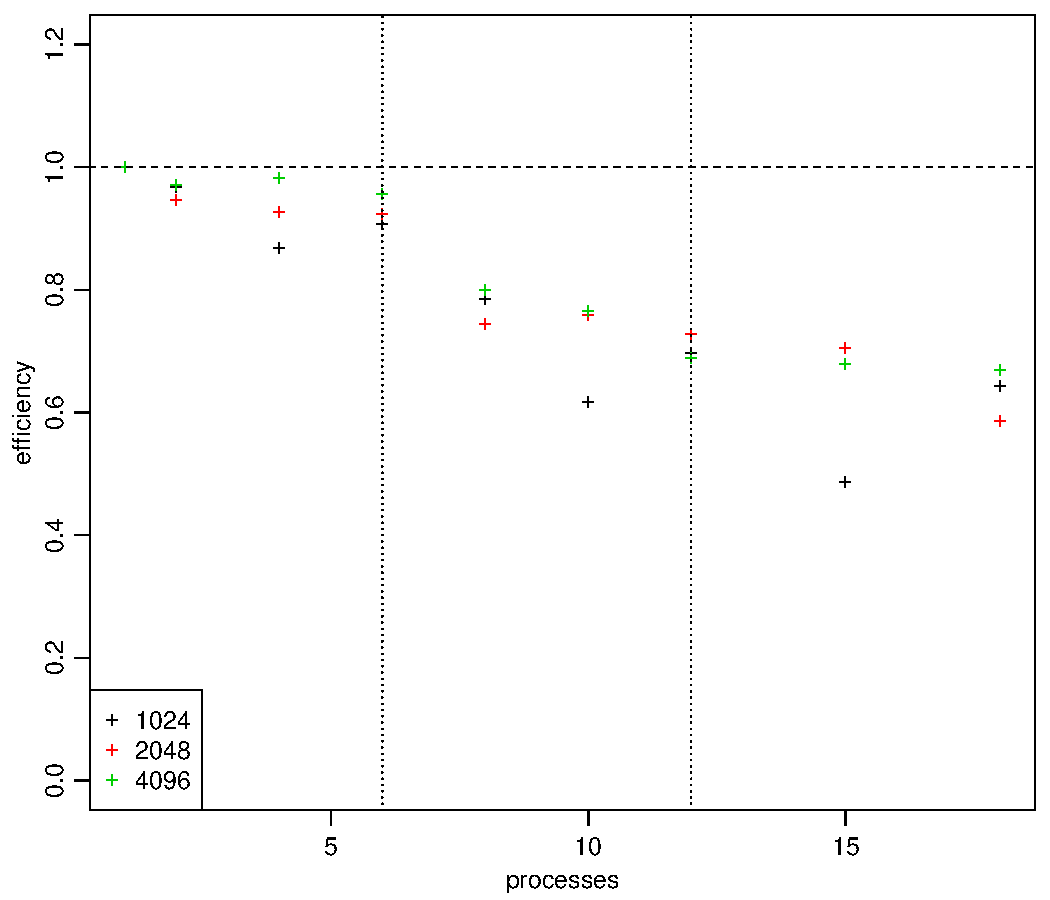
\includegraphics[width=\textwidth]{./Figures/taskbEfficiencyProc2.pdf}
  \end{subfigure}
          %(or a blank line to force the subfigure onto a new line)
  \vspace{1\baselineskip}
  \caption{Efficiency for running problem with different amount of processes. In the upper left figure each process has one thread, while in the upper right, each process has two treads. The problem is run on as few nodes as possible, and the processes are identically distributed among the nodes. There are drawn vertical lines to show when a new node is utilized, and a horizontal line at 1. The problem size $n$ is specified in the plots. In the bottom figure only one MPI process is run per node. Between 1 and 12 threads are run on each node.}
  \label{fig:Efficiency}
\end{figure}
%
\begin{figure}[h!]
  \centering
  \begin{subfigure}[b]{0.48\textwidth}
    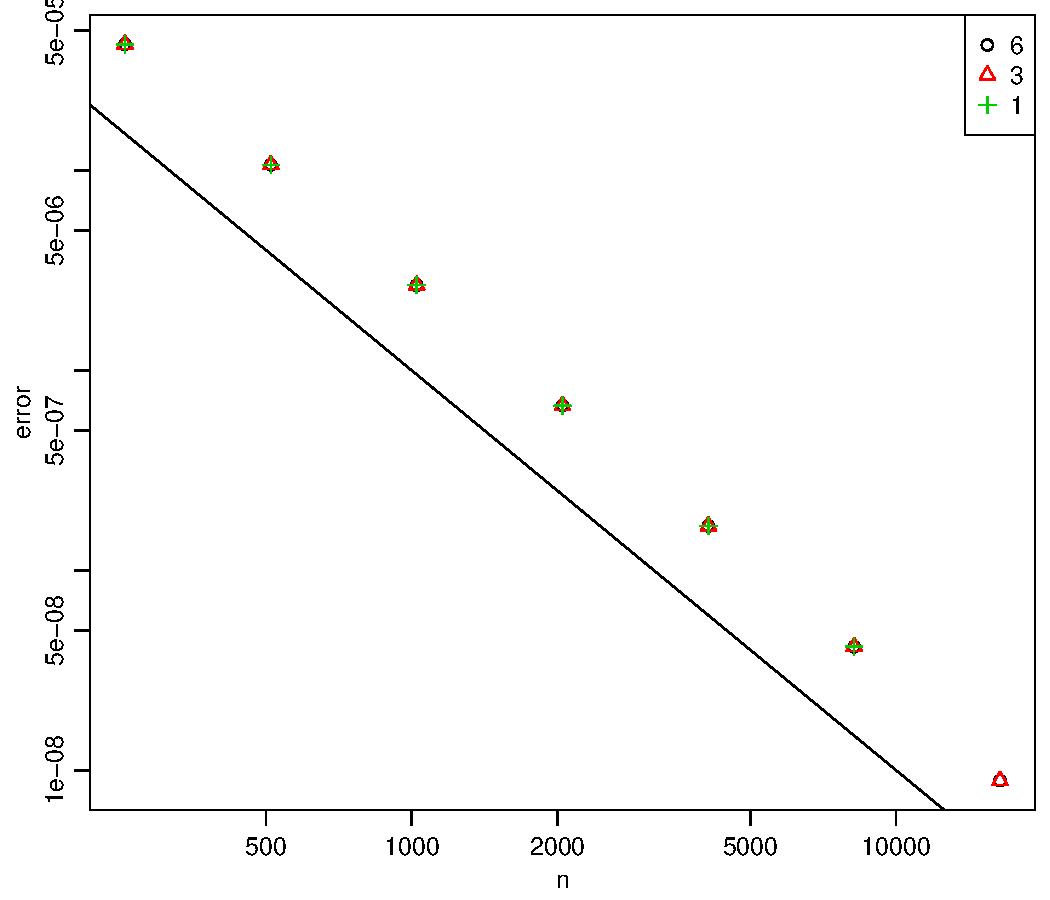
\includegraphics[width=\textwidth]{./Figures/errVsn.pdf}
  \end{subfigure}%
  \quad
  \begin{subfigure}[b]{0.48\textwidth}
    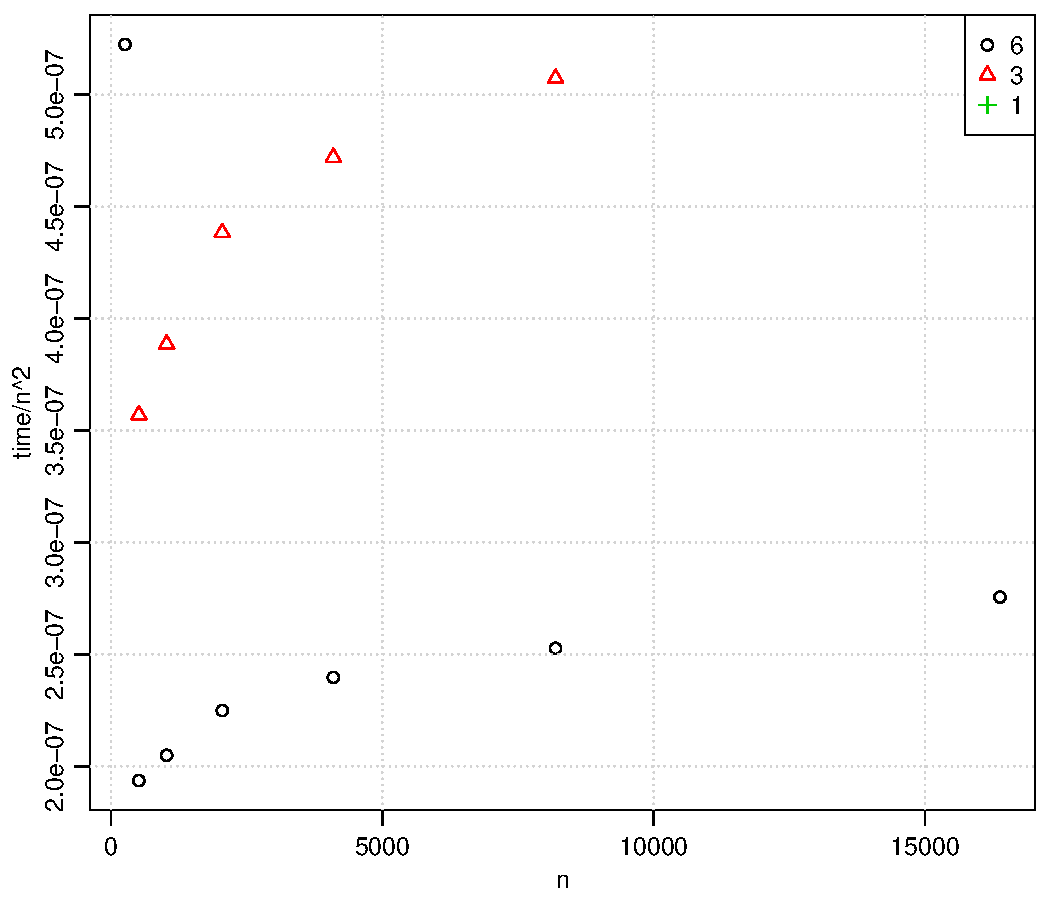
\includegraphics[width=\textwidth]{./Figures/timeOverN2Vsn.pdf}
  \end{subfigure}
          %(or a blank line to force the subfigure onto a new line)
  \vspace{1\baselineskip}
  \caption{The left figure shows a loglog plot of the error as function of $n$. A reference line with slope $-2$ is drawn. The problem is run on two threads, with the number of processes specified in the legend. Only one node is used. The right figure hows $time/n^2$.}
  \label{fig:conv}
\end{figure}



\section{Analysis}

speedup calculations, theoretic and observed

\section{Discussion}

\subsection{Bottlenecks}

\subsection{The non-homogenous case}
If one were to solve the Poisson problem with non-homogenous boundary conditions ie. $u = g(x) $ on $\partial \Omega$, 
some minor modifications would have to be done. 
The matrix system that is generated through this algorithm does not include the effect of the boundary elements, 
and in practice this is the same as assuming that they are iqual zero. The second order differential operator on the elements 
closest to the boundary are on the form 
\begin{equation}
	-\frac{\partial^2 u_{i,j}}{\partial x^2} = -\frac{u_{i-1,j}-2u_{i,j}}{h^2}
\end{equation}
The incrementations of $i,j$ will depend on which boundary the element is close to, but the form of the operator is nevertheless the same.
The effect on equation REF MAIN MATRIX EQ is that the boundary element is added to the left side.
In the homogenous case this does not affect the numerical algorithm, but in the non-homogenous case the boundary value needs to be added to the 
right hand side as well. This is implemented before the FST is done and does not have any impact on the parallel implementation. 
\subsection{Variations in the loading function $f$}
The loading function simply needs to be evaluated in all the grid points and multiplied by the steplength, before the 
FST-procedure starts. The only thing that will differ from the serial code is the displacement each process have.

\subsection{Variations in the domain $\Omega$}
By defining the domain $\Omega = (0,L_x)\times(0,L_y)$ but keeping the same number of grid points in each direction 
the discretization of the laplacian operator would be changed. In the unit square the discrete laplacian is defined as 
\begin{equation}
	\Delta u_{i,j} = \frac{u_{i-1,j}-2u_{i,j}+u_{i+1,j}}{h^2}+\frac{u_{i,j-1}-2u_{i,j}+u_{i,j+1}}{h^2}.
\end{equation}
In the new domain the operator would be defined as  
\begin{equation}
	\Delta u_{i,j} = \frac{u_{i-1,j}-2u_{i,j}+u_{i+1,j}}{h_x^2}+\frac{u_{i,j-1}-2u_{i,j}+u_{i,j+1}}{h_y^2}.
\end{equation}
Where $h_x=L_x/n$ and $h_y=L_y/n$ defines the new steplengths in each direction. Notice that the infamous 5-point formula now takes quite a 
different form and some rewriting is necessary. 
The diagonalized matrix system will now end up looking as 
\begin{equation}
	\left( \frac{1}{h_x^2}\underline{T} \; \underline{U}+\frac{1}{h_y^2}\underline{U}\; \underline{T} \right) _{i,j}=f_{i,j}
\end{equation}

By continuing the diagonalization procedure st. $\underline{T}=\underline{Q}\;\underline{\Lambda}\;\underline{Q}^T $
and defining $\underline{\tilde{U}}= \underline{Q}^T\;\underline{U}\;\underline{Q}$ one is left with the matrix system 

\begin{equation}
	\frac{1}{h_x^2}\underline{\Lambda} \; \underline{\tilde{U}}+\frac{1}{h_y^2}\underline{\tilde{U}}\; \underline{\Lambda} =\underline{\tilde{F}}.
\end{equation}

Notice that the right hand side can not be initially multiplied with the steplength $h^2$ since the two terms on the left hand side
now have different coefficients. This has to be done in step 2 of the algorithm, and would be implemented in the following way; 

\begin{equation}
	\tilde{u}_{i,j} = \frac{\tilde{f}_{i,j}}{\lambda_i/h_x+\lambda_j/h_y}.
\end{equation}

The last part of the algorithm would not need any further changing.
\end{document}

